\subsection{Diagrammi delle classi del Controller}
			\subsubsection{Package UserInputManager}
			\begin{figure}[h!]
			\begin{center}
				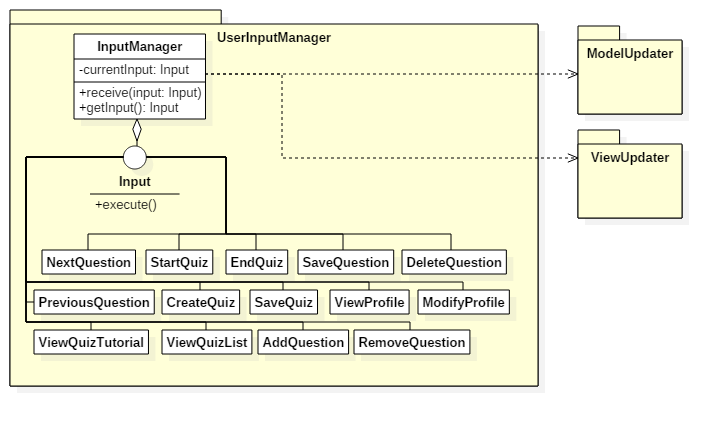
\includegraphics[scale=0.65]{../images/UserInputManagerClass.png}
				\caption{Diagramma delle classi del package UserInputManager}
			\end{center}
			\end{figure}

			\subsubsubsection{Classe InputManager}
			La classe implementa, con riferimento al pattern \emph{Command}, il componente Invoker del Command. In questo modo il trattamento degli input viene disaccoppiato dalle componenti che ne eseguiranno le richieste.
			\begin{itemize}
				\item\textbf{Funzione del componente}: riceve gli input dalla View e delega alle componenti del package Updaters la loro risoluzione.
				\item\textbf{Relazione d'uso di altre componenti}: si interfaccia con il package Updaters (che sono i suoi \emph{Receivers}) e con il package View dal quale riceve gli input.
				\item\textbf{Attività svolte e dati trattati}: questa classe possiede operazioni per ricevere e indirizzare ai giusti componenti gli input che le arrivano dalla View.
			\end{itemize}
			
			\subsubsubsection{Interfaccia Input}
			L'interfaccia implementa l'interfaccia di esecuzione delle richieste; con riferimento al pattern \emph{Command}, essa corrisponde alla classe Command. Quest'implementazione permette di aggiungere facilmente nuovi tipi di Input (concretizzazioni del Command).
			\begin{itemize}
				\item\textbf{Funzione del componente}: interfaccia di base degli input.
				\item\textbf{Relazione d'uso di altre componenti}: viene concretizzata in più sottoclassi. Oggetti delle sue sottoclassi vengono creati da View::Sender. Le sottoclassi concrete s'interfacciano con Updaters::ViewUpdater e Updaters::ModelUpdater.
				\item\textbf{Attività svolte e dati trattati}: definisce il contratto di ogni classe di tipo Input. Le classi concrete s'interfacciano con le classi del package Updaters in modo specializzato per ogni input.
				\item\textbf{Concretizzazioni}: Attualmente l'interfaccia Input viene concretizzata nelle seguenti sottoclassi (paragonabili, con riferimento al pattern \emph{Command}, a classi di tipo\emph{ConcreteCommand}), così definite:
				\begin{itemize}
				\item\textit{CreateQuiz}: richiede l'interfaccia per la creazione di un nuovo questionario.
				\item\textit{AddQuestion}: richiede di aggiungere una domanda al questionario in creazione.
				\item\textit{RemoveQuestion}: richiede di rimuovere una domanda precedentemente aggiunta nel questionario in creazione.
				\item\textit{SaveQuiz}: richiede di salvare un nuovo questionario appena creato.
				\item\textit{CreateQuestion}: richiede l'interfaccia per la creazione di una nuova domanda.
				\item\textit{SaveQuestion}: richiede di salvare nel sistema una nuova domanda.
				\item\textit{DeleteQuestion}: richiede di cancellare dal sistema una domanda precedentemente creata.
				\item\textit{ChooseQuiz}: richiede di caricare e presentare all'utente il quiz scelto.
				\item\textit{StartQuiz}: richiede di iniziare lo svolgimento di un quiz scelto.
				\item\textit{NextQuestion}: richiede la domanda successiva in un quiz.
				\item\textit{PreviousQuestion}: richiede la domanda precedente in un quiz.
				\item\textit{EndQuiz}: richiede di consegnare un quiz svolto completamente o in parte.
				\item\textit{ViewProfile}: richiede la pagina di visualizzazione del profilo utente.
				\item\textit{UpdateProfile}: richiede di modificare le informazioni nel profilo utente.
				\item\textit{ViewQMLTutorial}: richiede la visualizzazione del manuale utente QML.
				\item\textit{ViewQuizList}: richiede la visualizzazione di una lista di quiz.
				\end{itemize}
			\end{itemize}

			\subsubsection{Package Updaters}
			\begin{figure}[h!]
			\begin{center}
				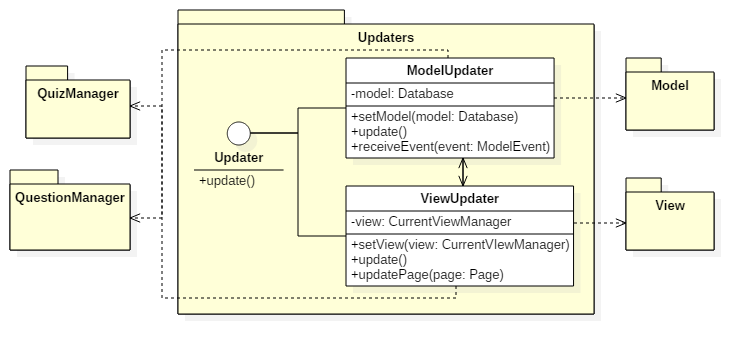
\includegraphics[scale=0.65]{../images/UpdatersClass.png}
				\caption{Diagramma delle classi del package Updaters}
			\end{center}
			\end{figure}
			\subsubsubsection{Interfaccia Updater}
			\begin{itemize}
				\item\textbf{Funzione del componente}: definisce le operazioni di base che andranno implementate nelle sottoclassi.
				\item\textbf{Relazione d'uso di altre componenti}: viene concretizzata in ViewUpdater e ModelUpdater.
				\item\textbf{Attività svolte e dati trattati}: nessuno.
			\end{itemize}
			
			\subsubsubsection{Classe ModelUpdater}
			\begin{itemize}
				\item\textbf{Funzione del componente}: inoltra al Model i dati da salvare su database. Riceve eventi dal Database.
				\item\textbf{Relazione d'uso di altre componenti}: collabora con le classi ViewUpdater, QuizManager e QuestionManager e s'interfaccia con la classe Database del Model esterna al package Presenter.
				\item\textbf{Attività svolte e dati trattati}: possiede un riferimento al Model e ne riceve gli eventi; tali eventi possono comportare l'aggiornamento della View, in tal caso collabora con la classe ViewUpdater. E' il \emph{Receiver} degli input che modificano il Model. Alcuni input possono richiedere la sua collaborazione con le classi QuizManager e QuestionManager.
			\end{itemize}

			\subsubsubsection{Classe ViewUpdater}
			\begin{itemize}
				\item\textbf{Funzione del componente}: è responsabile dell'aggiornamento della View rispetto agli input utente e rispetto alle modifiche del Model. E' il \emph{Receiver} degli input che modificano la View.
				\item\textbf{Relazione d'uso di altre componenti}: s'interfaccia con le classi ViewUpdater, QuizManager e QuestionManager e con le classi del package View.
				\item\textbf{Attività svolte e dati trattati}: la componente può ricevere input che non necessitano di interazione col Model; in tal caso provvede direttamente all'aggiornamento della View. Se è richiesta interazione col Model essa interagisce con la classe ModelUpdater. Alcuni input possono richiedere la sua collaborazione con le classi QuizManager e QuestionManager.
			\end{itemize}
			\newpage
			
			\subsubsection{Package QuestionManager}	
			Il package fa uso del design pattern \emph{Abstract Factory}.
			\begin{figure}[h!]
			\begin{center}
				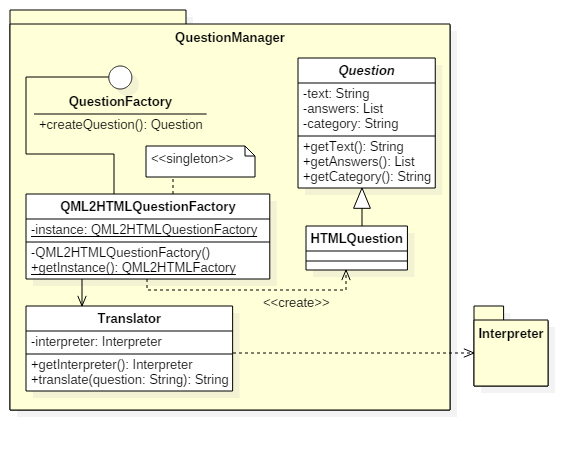
\includegraphics[scale=0.65]{../images/QuestionManagerClass.png}
				\caption{Diagramma delle classi del package QuestionManager}
			\end{center}
			\end{figure}
			\subsubsubsection{Interfaccia QuestionFactory}
			\begin{itemize}
				\item\textbf{Funzione del componente}: interfaccia di base delle Factory di tipi Question.
				\item\textbf{Relazione d'uso di altre componenti}: può essere concretizzata in diversi tipi di QuestionFactory.
				\item\textbf{Attività svolte e dati trattati}: definisce il contratto delle factory Question, cioè le operazioni di costruzione di Question che saranno definite in ogni concretizzazione.
			\end{itemize}
			
			\subsubsubsection{Classe astratta Question}
			\begin{itemize}
				\item\textbf{Funzione del componente}: classe di base del tipo Question.
				\item\textbf{Relazione d'uso di altre componenti}: può essere concretizzata in diversi tipi di Question.
				\item\textbf{Attività svolte e dati trattati}: definisce il contratto generale delle Question, cioè le loro operazioni e dati.
			\end{itemize}
			
			\subsubsubsection{Classe QML2HTMLQuestionFactory}
			La classe QML2HTMLQuestionFactory è un \emph{singleton}.
			\begin{itemize}
				\item\textbf{Funzione del componente}: crea oggetti di tipo HTMLQuestion.
				\item\textbf{Relazione d'uso di altre componenti}: è concretizzazione della classe QuestionFactory. Crea oggetti HTMLQuestion. Si interfaccia con la classe Translator.
				\item\textbf{Attività svolte e dati trattati}: crea su richiesta oggetti di tipo HTMLQuestion, delegando la traduzione del codice QML alla classe Translator.
			\end{itemize}
			
			\subsubsubsection{Classe HTMLQuestion}	
			\begin{itemize}
				\item\textbf{Funzione del componente}: rappresenta una domanda in formato HTML.
				\item\textbf{Relazione d'uso di altre componenti}: è concretizzazione di Question.
				\item\textbf{Attività svolte e dati trattati}: eredita e specializza le funzionalità dell'interfaccia Question.
			\end{itemize}
			
			\subsubsubsection{Classe Translator}
			\begin{itemize}
				\item\textbf{Funzione del componente}: s'interfaccia con le componenti del package Interpreter per la traduzione di quesiti QML in HTML.
				\item\textbf{Relazione d'uso di altre componenti}: collabora con le interfacce Interpreter e InterpreterFactory.
				\item\textbf{Attività svolte e dati trattati}: riceve dalla classe ViewUpdater le richieste di traduzione e il codice QML da tradurre. Attraverso la factory InterpreterFactory (una sua concretizzazione) costruisce un Interpreter concreto e lo utilizza per la traduzione del codice. L'esito della traduzione viene reso disponibile a ViewUpdater.
			\end{itemize}
			\newpage
			
			\subsubsection{Package QuizManager}
			Il package fa uso del design pattern \emph{Builder}.
			\begin{figure}[h!]
			\begin{center}
				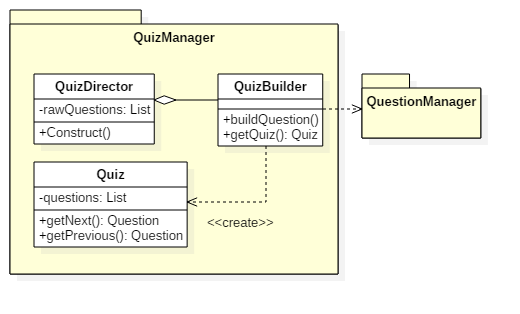
\includegraphics[scale=0.65]{../images/QuizManagerClass.png}
				\caption{Diagramma delle classi del package QuizManager}
			\end{center}
			\end{figure}
			\subsubsubsection{Classe QuizDirector}
			\begin{itemize}
			\item\textbf{Funzione del componente}: è responsabile della costruzione di un oggetto di tipo Quiz.
				\item\textbf{Relazione d'uso di altre componenti}: utilizza la classe QuizBuilder.
				\item\textbf{Attività svolte e dati trattati}: la classe, a partire da un set di domande (in questo caso in QML), utilizza il Builder per costruire un Quiz.ì
			\end{itemize}
			
			\subsubsubsection{Classe QuizBuilder}
			\begin{itemize}
			\item\textbf{Funzione del componente}: Costruisce domanda per domanda un questionario.
				\item\textbf{Relazione d'uso di altre componenti}: interagisce con il package QuestionManager.
				\item\textbf{Attività svolte e dati trattati}: Costruisce passo pe r passo un oggetto di tipo Quiz. Si appoggia al package QuestionManager per la creazione delle singole domande.
			\end{itemize}
			
			\subsubsubsection{Classe Quiz}
			\begin{itemize}
			\item\textbf{Funzione del componente}: la classe rappresenta un Quiz, una raccolta di domande.
				\item\textbf{Relazione d'uso di altre componenti}: nessuna.
				\item\textbf{Attività svolte e dati trattati}: la classe possiede i dati e fornisce le operazioni necessaria alla fruizione di un Quiz.
			\end{itemize}
			\clearpage			
			
			\subsubsection{Package Interpreter}
			\begin{figure}[h!]
			\begin{center}
				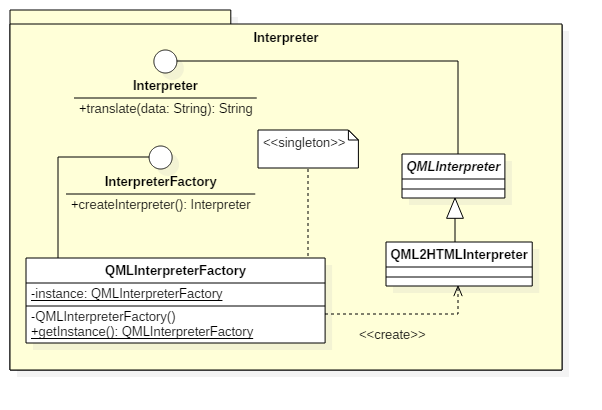
\includegraphics[scale=0.65]{../images/InterpreterClass.png}
				\caption{Diagramma delle classi del package Interpreter}
			\end{center}
			\end{figure}
			\subsubsubsection{Interfaccia Interpreter}
			\begin{itemize}
				\item\textbf{Funzione del componente}: interfaccia di base del tipo Interpreter.
				\item\textbf{Relazione d'uso di altre componenti}: può essere concretizzata in diversi tipi di Interpreter. Viene riferita dalla classe Translator.
				\item\textbf{Attività svolte e dati trattati}: definisce il contratto degli Interpreter, cioè le operazioni di traduzione che saranno definite in ogni concretizzazione.
			\end{itemize}
			\subsubsubsection{Interfaccia InterpreterFactory}
			\begin{itemize}
				\item\textbf{Funzione del componente}: interfaccia di base delle Factory di tipi Interpreter.
				\item\textbf{Relazione d'uso di altre componenti}: può essere concretizzata in diversi tipi di InterpreterFactory. Viene riferita dalla classe Translator.
				\item\textbf{Attività svolte e dati trattati}: definisce il contratto delle factory, cioè le operazioni di costruzione di Interpreter che saranno definite in ogni concretizzazione.
			\end{itemize}
			\subsubsubsection{Classe QMLInterpreterFactory}
			La classe QMLInterpreterFactory è un \emph{singleton}.
			\begin{itemize}
				\item\textbf{Funzione del componente}: crea oggetti di tipo QMLInterpreter.
				\item\textbf{Relazione d'uso di altre componenti}: è concretizzazione della classe InterpreterFactory. Crea oggetti QMLInterpreter.
				\item\textbf{Attività svolte e dati trattati}: crea su richiesta oggetti di tipo QMLInterpreter.
			\end{itemize}
			\subsubsubsection{Classe QMLInterpreter}
			\begin{itemize}
				\item\textbf{Funzione del componente}: classe astratta che rappresenta gli Interpreter che traducono codice QML in un altro formato.
				\item\textbf{Relazione d'uso di altre componenti}: è sottotipo di Interpreter. Può essere concretizzata in più tipi di QMLInterpreter.
				\item\textbf{Attività svolte e dati trattati}: definisce il contratto dei QMLInterpreter, cioè le operazioni di traduzione da QML verso altri linguaggi.
			\end{itemize}
			\subsubsubsection{Classe QML2HTMLInterpreter}	
			\begin{itemize}
				\item\textbf{Funzione del componente}: traduce codice QML in codice HTML.
				\item\textbf{Relazione d'uso di altre componenti}: è concretizzazione di QMLInterpreter.
				\item\textbf{Attività svolte e dati trattati}: riceve in input domande in QML e le traduce in codice HTML visualizzabile da browser.
			\end{itemize}
			\newpage